\section{Introduction}
\input{figures/database_long_tail.tex}
China, with its extensive and culturally rich history, has accumulated a vast array of historical documents spanning centuries of scholarship, governance, and literary expression. These documents offer incomparable academic and artistic value, presenting essential insights into linguistics, cultural anthropology, and social development. Consequently, there has been an upsurge of research interest directed towards the analysis and recognition of historical documents~\cite{jinic21,hde,obc306}. As researchers delve deeper into this field, new methodologies have been developed to contend with the inherent complexities that arise from the condition and content of such documents.

Historical texts often pose challenges distinct from modern text recognition, largely due to the presence of severe physical degradation. Stains, tears, and ink bleeding result from the natural aging process or prolonged exposure to environmental factors. These forms of damage cause substantial visual distortions in the character glyphs, making accurate recognition difficult even for advanced methods~\cite{Hong2021, Dou2021}. Additionally, scribal variations, regional styles, and calligraphic differences across dynasties create a remarkable diversity in character shapes. This complexity further necessitates specialized modeling strategies that account for inconsistent ink intensities and complex stroke structures, which are seldom seen in modern documents. This uniqueness of historical documents also emphasizes the importance of domain knowledge and domain-specific model architectures that can robustly handle the variety of possible degradations.

Aside from the visual difficulties introduced by document quality, another key issue in historical document recognition originates from the distribution of the data itself, where certain characters are extremely frequent while others scarcely appear~\cite{obcmk2}. This long-tailed character occurrence distribution presents a formidable obstacle, as it forces models to overfit high-frequency characters while largely ignoring the underrepresented, albeit significant, tail characters. Although the long-tailed distribution also affects other text recognition tasks~\cite{fudanvi}, historical document recognition manifests a substantially higher degree of ``longtailness,'' measured by the Gini Coefficient~\cite{tailsurvey} (see Figure~\ref{fig:moretailed}). This metric highlights the pronounced skew in historical texts, wherein a small set of characters occupies the majority of instances. Consequently, designing methods that can accommodate these skewed distributions is crucial for achieving reliable recognition performance.

Moreover, new characters in test data tend to be situated at the distribution's tail~\cite{jinic21}, effectively combining open-set recognition with long-tail challenges. The emergence of these previously unseen characters, often archaic or region-specific, can significantly degrade the performance of models trained solely on common categories. In such scenarios, robust generalization to novel classes is not merely beneficial but essential, as the inability to correctly identify or interpret new characters could jeopardize critical historical interpretations. Recent research efforts have thus begun to investigate strategies that explicitly encode prior knowledge or structural information to mitigate the negative effects of sparse tail samples~\cite{Tang2022}.

To address this confluence of obstacles, existing methods exploit the radical information of each character, capitalizing on the fact that radicals often act as semantic or phonetic building blocks~\cite{denseran}. Since individual radicals may appear across both head and tail classes, the utilization of radical information has shown promising generalization capabilities for recognizing previously unseen characters~\cite{fewran,zhang20pr}. By breaking down unfamiliar glyphs into known components, radical-based methods can approximate the correct representation of characters appearing in the tail. On the other hand, Zhang et al.~\cite{sanicdar23} proved that leveraging component information significantly enhances tail class performance by effectively sharing knowledge between more common and extremely rare characters. Despite the effectiveness of these techniques, a significant limitation arises from their reliance on radical-level annotations, which require laborious expert labeling for each character’s constituent parts. As a result, annotation costs balloon in large-scale projects, and difficulties arise in transferring such methods to different scripts or new sets of characters.

In this work, we propose a strategy that aims to circumvent the requirement for labor-intensive radical annotations by adopting a visual matching approach~\cite{vsdf}. Our goal is to continue exploiting the similarity among character components while implicitly emphasizing detailed feature modeling. Specifically, we develop a novel spindle backbone network that allocates an increased number of parameters to the layers responsible for capturing component-level features, a design choice motivated by the desire to amplify the network’s sensitivity to the subtleties of shared parts across characters. Inspired by insights from mobile neural network architectures~\cite{mobile} and investigations into feature dissection~\cite{dissection}, the spindle backbone focuses on expanding the capacity of middle layers (conv2 and conv3), which are crucial for extracting mid-level texture-like features. We argue that these middle layers are inherently better at representing the strokes and partial forms characteristic of radicals or sub-character components. By contrast, high-frequency signals in shallow layers are often detrimental to generalization~\cite{hfharm,hffilter}, so our design refrains from widening the shallowest layers. 

In parallel, the deeper layers of the network are streamlined to sustain a compact overall parameter footprint, thus preserving both high inference speed and reduced VRAM usage. This balanced approach ensures that the network remains deployable in resource-constrained environments such as digital libraries and cultural heritage archives that maintain large-scale digitization workflows. Combining these elements, the spindle backbone emerges as a design that strategically prioritizes mid-level features without significantly inflating computational cost.

Summarizing these motivations, we present a spindle network with narrow shallow layers and narrow deep layers but wider middle layers, enabling stronger learning of stroke-like structures that can be reused across head, tail, and even novel classes. In addition, the Radical Residual Module (RSM) is incorporated to further boost the representational power of the features corresponding to character radicals. By integrating both spatial and channel attention while drawing upon prior knowledge of 265 common radical templates, the RSM can guide the network to focus on relevant spatial regions more effectively. This enhanced spatial attention ultimately contributes to improved discrimination of fine-grained radical or stroke patterns, thus elevating recognition performance for both seen and unseen classes.

The RSM integrates spatial attention mechanisms that attend to local character regions where radicals are likely to be found, and it uses channel attention to calibrate the importance of different feature maps. These processes benefit from the partial supervision derived from the radical templates, which provide gentle guidance in highlighting areas of interest. In doing so, the network is naturally steered to emphasize consistent component features that are characteristic of radicals across an extensive range of text samples. As a result, the representation of novel characters is bolstered, and the tail classes witness improvements in recognition accuracy that are especially vital in historical document contexts where annotated data is scarce or unevenly distributed.

We conducted architectural ablation studies to verify that the spindle design outperforms both the traditional pyramid design and the reverse pyramid design in terms of overall accuracy and robustness. Experimental outcomes reveal that our emphasis on mid-level feature expansion aligns with the structural complexities of historical documents, allowing better generalization to atypical or damaged characters. This observed superiority underscores the practical value of carefully tailoring the network architecture to address the multiple demands of historical text recognition, where visual degradation, long-tail distributions, and open-set challenges frequently coexist~\cite{Bai2023}.

As a structural-knowledge-free approach, the proposed method also exhibits compelling recognition abilities when confronted with novel classes, significantly reducing the labor involved in adapting the model to newly uncovered historical materials or freshly excavated scripts. Empirically, our network's capacity to handle both head and tail classes sees consistent gains in experiments, reinforcing its applicability in large-scale digitization efforts that require not just sheer accuracy, but also the flexibility to accommodate continuous discoveries of rare and unknown characters. Ultimately, by sidestepping expensive radical-level annotations while still capturing compositional character information, the proposed approach marks a step forward in making historical text recognition more scalable, comprehensive, and adept at handling the myriad challenges ingrained in ancient manuscripts.

In summary, the main contributions of this paper can be considered as follows:
\begin{itemize}
\item we introduce the Radical Residual Module (RSM), which strategically exploits the intrinsic similarity among character radicals to enhance recognition performance, especially for novel or infrequently appearing characters. By incorporating both spatial and channel attention mechanisms, the RSM guides the model to focus on shared substructures that transcend individual glyphs, thereby improving the system’s capacity to generalize beyond the training set. 
\item Building upon this radical-aware framework, we then propose a spindle network designed to deepen the extraction of character components. This architecture widens the intermediate layers where sub-character features and texture-like patterns are most salient, leveraging commonalities across various components and improving the representation of complex or degraded characters. The enhanced capacity in mid-level layers amplifies the model’s ability to capture nuanced details, leading to tangible gains in recognizing unseen or rare glyphs and thus addressing the challenges posed by long-tailed distributions. 
\item we validate the effectiveness and versatility of our method through extensive experiments on three challenging Chinese ancient book datasets, namely TKH, MTH1000, and MTH1200. Empirical results clearly demonstrate that our approach achieves state-of-the-art performance in this domain, underscoring its practicality for large-scale historical document digitization. By integrating radical-informed cues with a balanced architectural design, our framework not only achieves higher accuracy but also exhibits robust generalization across both abundant and rare character classes.
\end{itemize}


\begin{figure*}[t]
    \begin{center}
    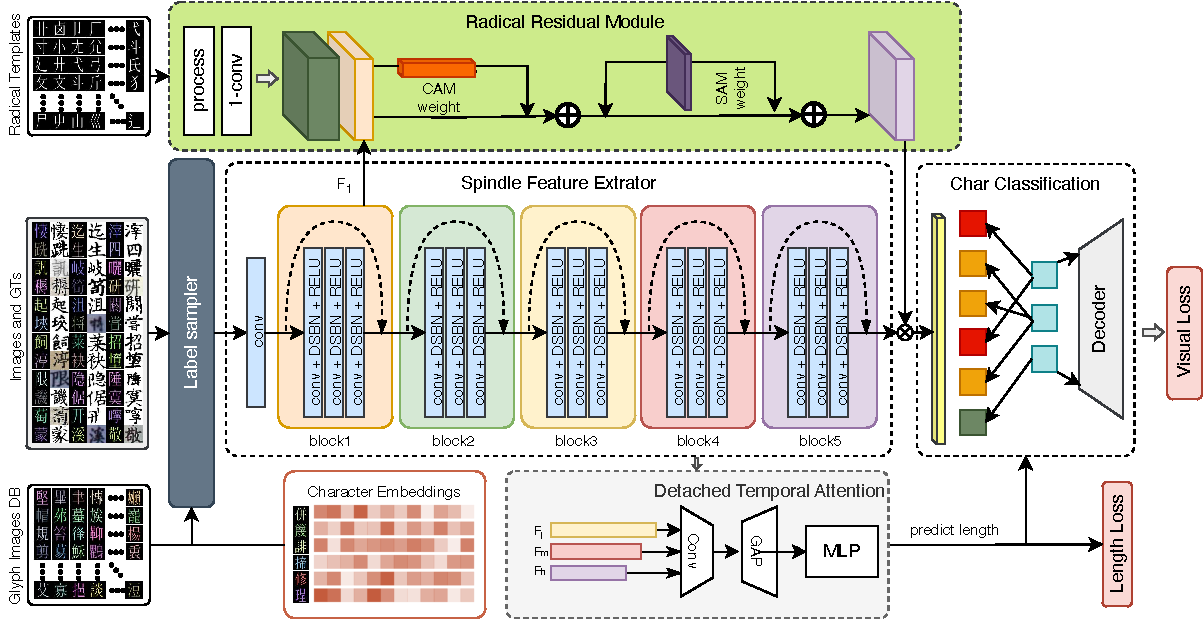
\includegraphics[width=1.0\linewidth]{figures/overall.pdf}
    \end{center}
    \caption{Overview. This framework is composed of four modules: a feature extraction module, a character length module, a decoder module, and a Radical Residual Module.}
    \label{fig:overall}
\end{figure*}
